
\section{Results}

Figure \ref{training_stats1} and \ref{training_stats2}  show the evolution of the loss, training and validation accuracy in the two experimental setups. Consistent results are observed across different folds ensuring robustness of this validation strategy. Note that, since gradient accumulation is used, the number of iterations is shown on the x-axis. The translation into epochs is:
\begin{equation}
    \text{Epochs} = \frac{\text{Iterations}}{\text{training set size}/\text{Batch size}}
\end{equation}

For example, in first setup the training set size is $1200\times0.6$ and batch size is $128$ which means that $5,6$ iterations correspond to 1 epoch. 

Note that the loss and the validation accuracy are respectively decreasing and increasing consistently over the training, which is a good sign that the model is learning the task without overfitting. 
Accuracy and confusion matrix are reported in Table \ref{res_tab1} \ref{res_tab2} and Figure \ref{conf_mat}. They consist in the averaged values over all the folds. Our model is performing better than current state of the art, with an accuracy of 91,66\% with the same experimentation setup of the other cited works.

Note that all the known models validated on BU3DFE are based on a two streams architecture (RGB (or grayscale) and Depth) with different fusion strategies and none of them is using the mesh directly. Looking at the confusion matrices, in the first setup, the worst performing class is Surprise. Note the high overlap between disgust-fear, fear-surprise and disgust-anger; this is because such expressions present similar features like open mouth and wide eyes for Fear-Surprise, or frowned eyebrows Disgust-Anger.  

In the second setup, considering also neutral class and lower intensity expressions, the worst performing class is the Neutral , probably because of the low number of neutral samples (only 100 samples) and the high similarity between neutral and lower intensity expressions.

CalD3r and MenD3s is also used for model validation, where the model outperform the Marcolin et al. network \cite{CalD3rMenD3s} from 58,30 to 65,11 (in the 6 classes setup, without surprise) and 62,50 when considering all 7 emotions. The comparison of results between the two datasets confirms that FER over posed datasets, like BU3DFE, is much easier task than over spontaneous dataset, like CalD3rMenD3s. In fact, Figure \ref{BU3DFE_stats} shows that the features extracted by the model on the BU3DFE dataset are very well separated since the posed expressions are more different from each other with respect to the spontaneous ones in CalD3rMenD3s analysed in Figure \ref{features_img}. 

\raggedbottom
\begin{figure}
    \centering
    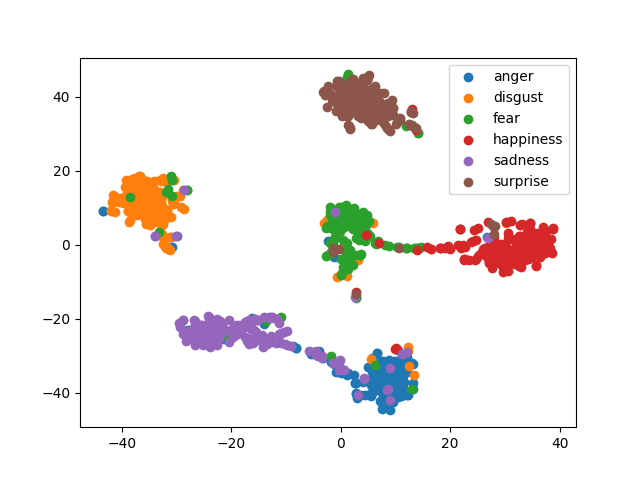
\includegraphics[width=1.1\columnwidth]{Images/BU3DFE_6_features.png}
    \caption{BU3DFE 6 classes features}
    \label{BU3DFE_stats}
\end{figure}

\begin{table}[H]
    \centering
    \captionsetup{justification=centering, width=0.8\columnwidth} % Adjust width as needed
    \caption{Results on BU3DFE (w/o Neutral class, 
    only 2 highest intensity levels, 60 subjects.
    Results averaged on 10 fold validation 100 times)} 
    \begin{tabular}{cccc}
    \hline
    Model & Year & Accuracy (\%)& Classes\\
    \hline
    MFEVIT \cite{RW_8D_MFEVIT} &2021 & 90,83& 6\\
    \hline
    CMANET \cite{RW_8B_CMANET} & 2022 & 90,24 & 6 \\
    \hline
    CMFN \cite{RW_9_CMFN} & 2023 & 88,91 & 6\\
    \hline
    AFNET \cite{RW_8A_AFNET} & 2023  & 90,08& 6\\
    \hline
    \textbf{This} &  2024  & 91,66& 6\\                                               
    \hline
    \end{tabular}
    \label{res_tab1}
\end{table}

\begin{table}[H]
    \centering
    \captionsetup{justification=centering, width=0.8\columnwidth} % Adjust width as needed
    \caption{Our benchmark on BU3DFE (Full dataset. Results averaged on 5 fold validation)} 
    \begin{tabular}{cccc}
    \hline
    Model & Year & Accuracy (\%)& Classes\\
    \hline
    \textbf{This} &  2024  & 87,6 & 7\\                                          
    \hline
    \end{tabular}
    \label{res_tab2}
\end{table}


\begin{figure*}[ht]
    \centering
    \begin{subfigure}{\textwidth} 
        \centering
        \begin{subfigure}{0.32\textwidth}
            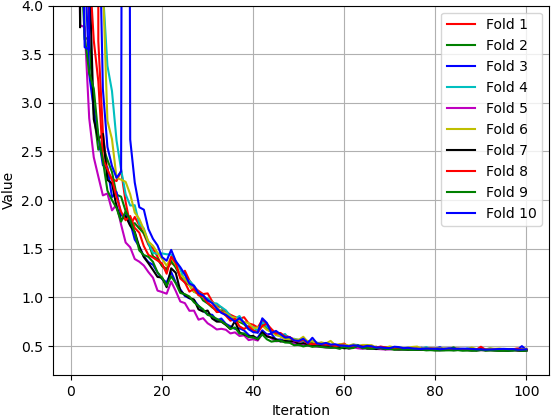
\includegraphics[width=\linewidth]{Images/training/BU3DFE_6_train_loss.png}
            \caption{Training Loss}
            \label{BU3DFE_6_train_loss}
        \end{subfigure}
        \begin{subfigure}{0.32\textwidth}
            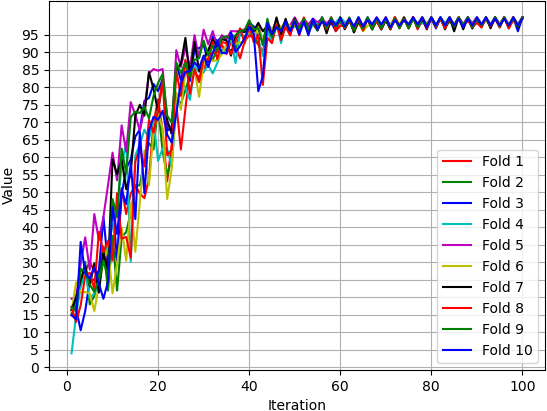
\includegraphics[width=\linewidth]{Images/training/BU3DFE_6_train_acc.png}
            \caption{Training Accuracy}
            \label{BU3DFE_6_train_acc}
        \end{subfigure}
        \begin{subfigure}{0.32\textwidth}
            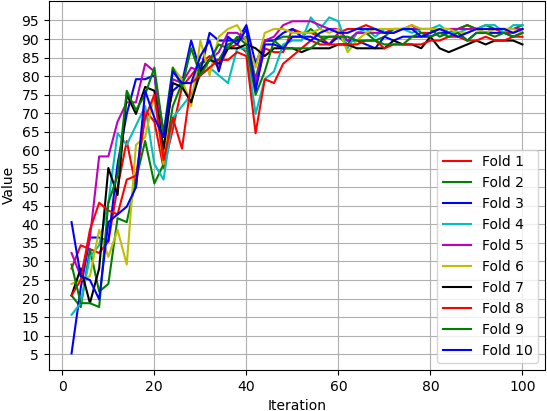
\includegraphics[width=\linewidth]{Images/training/BU3DFE_6_val_acc.png}
            \caption{Validation Accuracy}
            \label{BU3DFE_6_val_acc}
        \end{subfigure}
    \end{subfigure}
    \caption{Training and Validation Statistics for BU3DFE (w/o Neutral class, 
    only 2 highest intensity levels, 60 subjects). 90-10 validation over 1 repetition as an example.}
    \label{training_stats1}
\end{figure*}
\begin{figure*}[ht]
    \begin{subfigure}{\textwidth}
        \centering
        \begin{subfigure}{0.32\textwidth}
            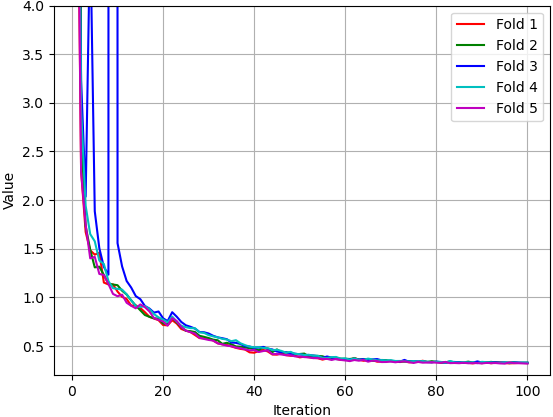
\includegraphics[width=\linewidth]{Images/training/BU3DFE_7_train_loss.png}
            \caption{Training Loss}
            \label{BU3DFE_7_train_loss}
        \end{subfigure}
        \begin{subfigure}{0.32\textwidth}
            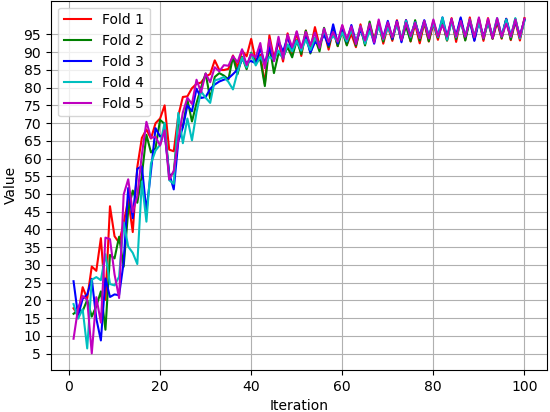
\includegraphics[width=\linewidth]{Images/training/BU3DFE_7_train_acc.png}
            \caption{Training Accuracy}
            \label{BU3DFE_7_train_acc}
        \end{subfigure}
        \begin{subfigure}{0.32\textwidth}
            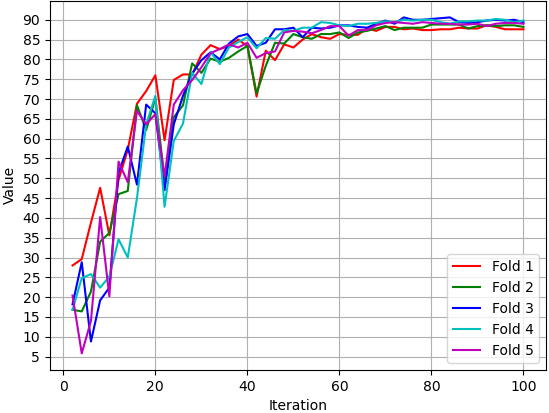
\includegraphics[width=\linewidth]{Images/training/BU3DFE_7_val_acc.png}
            \caption{Validation Accuracy}
            \label{BU3DFE_7_val_acc}
        \end{subfigure}
    \end{subfigure}
    \caption{Training and Validation Statistics for BU3DFE (Full dataset, 5 fold validation)}
    \label{training_stats2}
\end{figure*}




\begin{figure}[H]
    \centering
    \begin{subfigure}[t]{0.4\textwidth}
        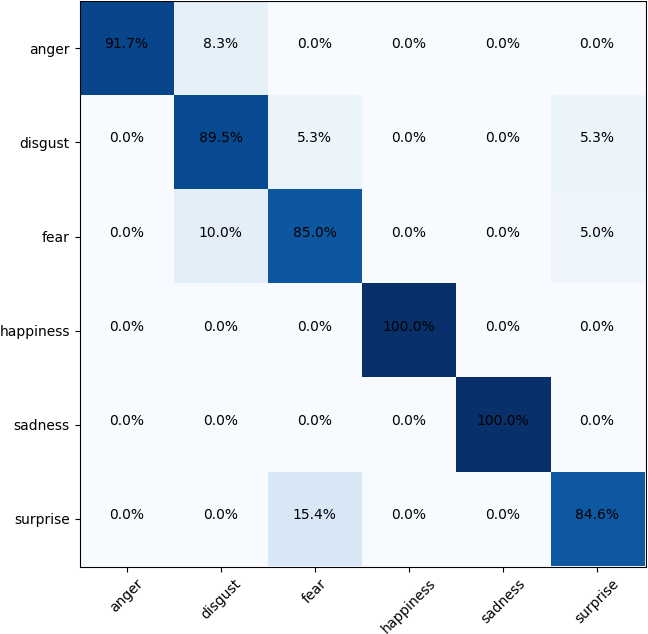
\includegraphics[width=\linewidth]{Images/conf_mat/conf_mat_BU3DFE_6_only_highest.png}
        \caption{w/o Neutral class, 
        only 2 highest intensity levels, 60 subjects. \\ Results averaged on 10 fold validation 100 times}
        \label{conf_mat_BU3DFE_6_only_highest}
        \vspace{0.2cm}
    \end{subfigure}
  
    \begin{subfigure}[t]{0.4\textwidth}
        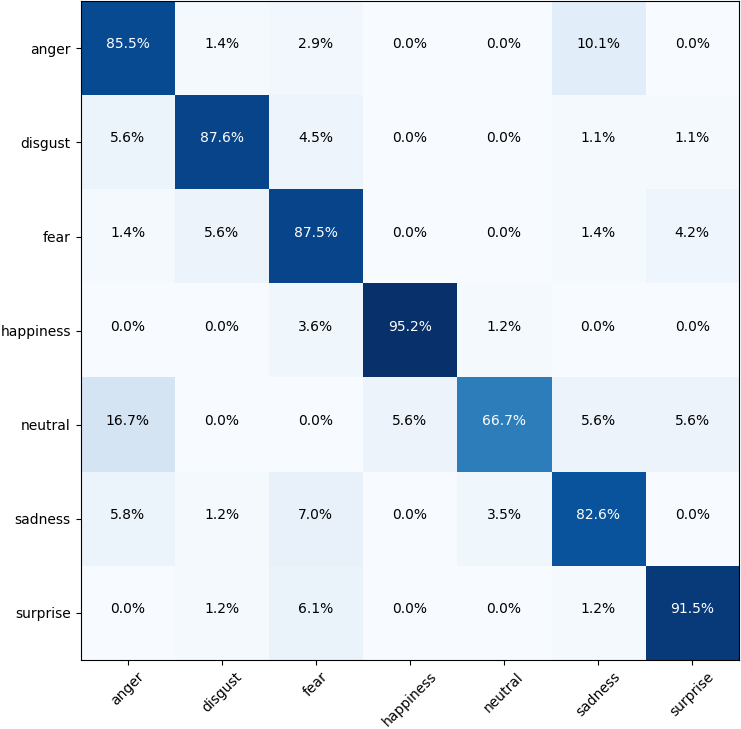
\includegraphics[width=\linewidth]{Images/conf_mat/conf_mat_BU3DFE_7.png}
        \caption{Full dataset. \\
        Results averaged on 5 fold validation}
        \label{BU3DFE 7 classes}
    \end{subfigure}
    \caption{BU3DFE Confusion Matrices. X-axis are the predicted class, Y-axis is the true class.}
    \label{conf_mat}
\end{figure}


    
   
\subsection{Attention analysis}
GRADCAM \cite{Gradcam} is used to visualize where the model is focusing on the input image to make the prediction. Gradcam computes the score of the target class at the output of a convolutional layer and then performs backpropagation using that score as a loss value. Figure \ref{heatmaps} shows the attention maps for 2 correctly classified validation samples per each class. As expected, note that the most informative regions, where the network poses more attention, are the eyebrows, eyes and mouth.


\begin{figure*}[ht]
    \centering
    % First row: Anger and Sadness
    \begin{subfigure}{0.45\textwidth}
        \centering
        \begin{subfigure}{0.45\textwidth}
            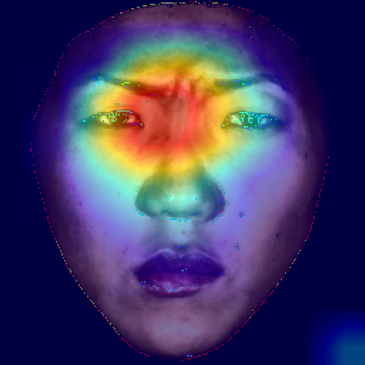
\includegraphics[width=\linewidth]{Images/Heatmaps/heatmap_anger_1.png}
        \end{subfigure}
        \begin{subfigure}{0.45\textwidth}
            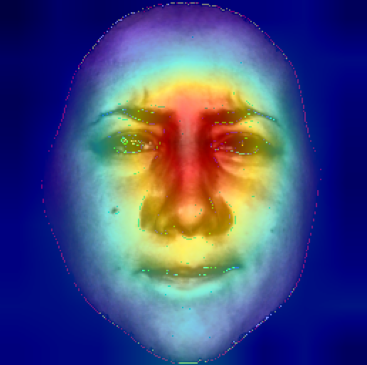
\includegraphics[width=\linewidth]{Images/Heatmaps/heatmap_anger_2.png}
        \end{subfigure}
        \caption{Anger}
    \end{subfigure}
    \hspace{0.05\textwidth} % Add horizontal space
    \begin{subfigure}{0.45\textwidth}
        \centering
        \begin{subfigure}{0.45\textwidth}
            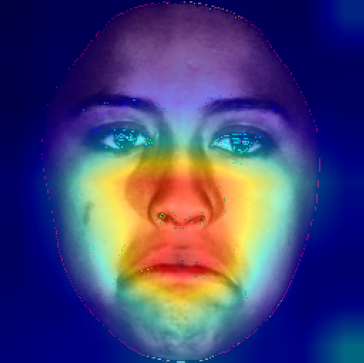
\includegraphics[width=\linewidth]{Images/Heatmaps/heatmap_sadness_1.png}
        \end{subfigure}
        \begin{subfigure}{0.45\textwidth}
            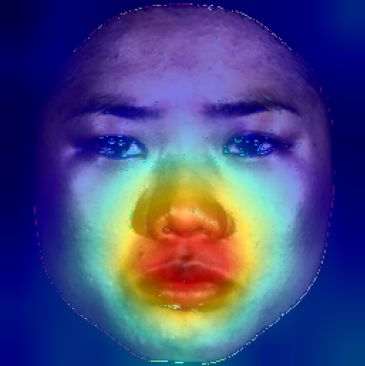
\includegraphics[width=\linewidth]{Images/Heatmaps/heatmap_sadness_2.png}
        \end{subfigure}
        \caption{Sadness}
    \end{subfigure}

    % Second row: Happiness and Fear
    \begin{subfigure}{0.45\textwidth}
        \centering
        \begin{subfigure}{0.45\textwidth}
            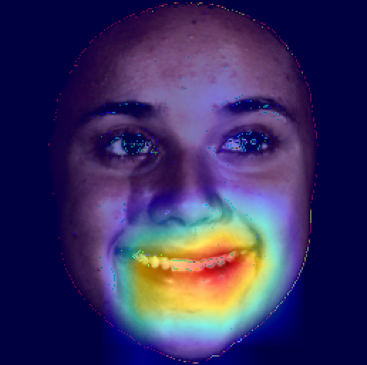
\includegraphics[width=\linewidth]{Images/Heatmaps/heatmap_happiness_1.png}
        \end{subfigure}
        \begin{subfigure}{0.45\textwidth}
            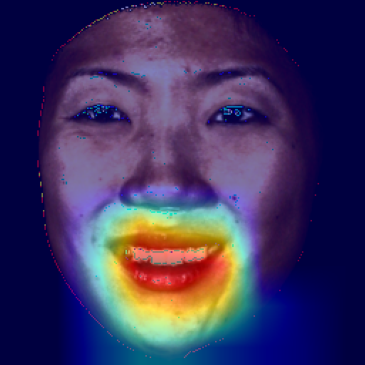
\includegraphics[width=\linewidth]{Images/Heatmaps/heatmap_happiness_2.png}
        \end{subfigure}
        \caption{Happiness}
    \end{subfigure}
    \hspace{0.05\textwidth} % Add horizontal space
    \begin{subfigure}{0.45\textwidth}
        \centering
        \begin{subfigure}{0.45\textwidth}
            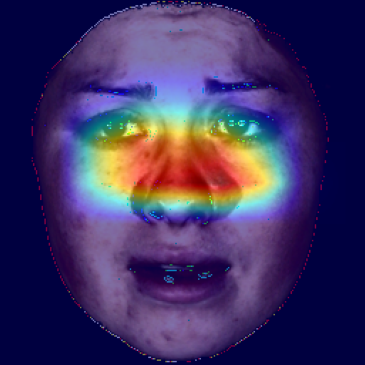
\includegraphics[width=\linewidth]{Images/Heatmaps/heatmap_fear_1.png}
        \end{subfigure}
        \begin{subfigure}{0.45\textwidth}
            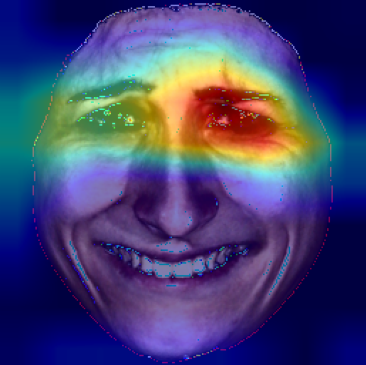
\includegraphics[width=\linewidth]{Images/Heatmaps/heatmap_fear_2.png}
        \end{subfigure}
        \caption{Fear}
    \end{subfigure}

    % Third row: Disgust and Surprise
    \begin{subfigure}{0.45\textwidth}
        \centering
        \begin{subfigure}{0.45\textwidth}
            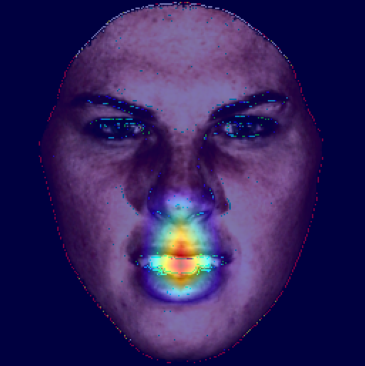
\includegraphics[width=\linewidth]{Images/Heatmaps/heatmap_disgust_1.png}
        \end{subfigure}
        \begin{subfigure}{0.45\textwidth}
            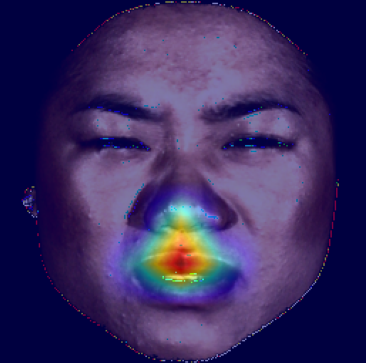
\includegraphics[width=\linewidth]{Images/Heatmaps/heatmap_disgust_2.png}
        \end{subfigure}
        \caption{Disgust}
    \end{subfigure}
    \hspace{0.05\textwidth} % Add horizontal space
    \begin{subfigure}{0.45\textwidth}
        \centering
        \begin{subfigure}{0.45\textwidth}
            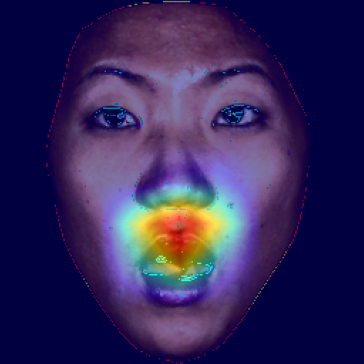
\includegraphics[width=\linewidth]{Images/Heatmaps/heatmap_surprise_1.png}
        \end{subfigure}
        \begin{subfigure}{0.45\textwidth}
            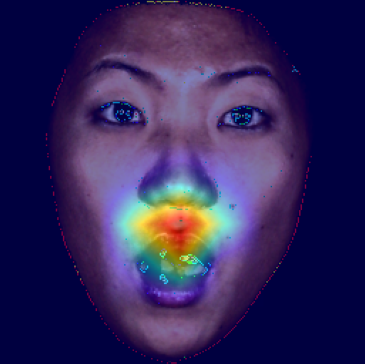
\includegraphics[width=\linewidth]{Images/Heatmaps/heatmap_surprise_2.png}
        \end{subfigure}
        \caption{Surprise}
    \end{subfigure}

    \caption{Heatmaps for each emotion class}
    \label{heatmaps}
\end{figure*}

\subsection{Modality Ablation}
The contribution of depth modality is now evaluated by training the model only using the RGB stream. The results shown in Table \ref{modality_ablation_tab} are referred to the same cross validation used for the previous experiments.

\begin{table}[H]
    \centering
    \caption{Modality Ablation}
    \begin{tabular}{cc}
    \hline
    Modality & Accuracy (\%)\\
    \hline
    RGB & 88,72\\
    \hline
    RGB+Depth & 91,66\\
    \hline
    \end{tabular}
    \label{modality_ablation_tab}
\end{table}

Note that the depth modality provides a significant improvement in the accuracy, confirming the importance of the depth information.

\subsection{Modules Ablation}
Table \ref{mod_abl_tab} compares the full model with and without final ViT encoder (which is substituted by a final AvgPooling), and without the Cross Modality Spatial Attention which is replaced with sum fusion between the features from the two modalities:

\begin{equation}
    \bm{p} = Softmax(MLP(AvgPool((\bm{X_{rgb}}) + (\bm{X_{depth}}))))
\end{equation}

\begin{table}[H]
    \centering
    \caption{Modules Ablation}  \label{mod_abl_tab}
    \begin{tabular}{ccc}
    \hline
    Cross Mod. Spatial Att. & ViT encoder & Accuracy(\%)\\
    \hline
    \ding{55} & \ding{55} &  87,25\\
     \hline
     \ding{55} & \checkmark &  88,17\\
    \hline
    \checkmark &\ding{55} & 91,45 \\
    \hline
    \checkmark &\checkmark & 91,66\\
    \hline
    \end{tabular}
\end{table}

Note the consistent drop in performance when not using the Cross Modality Spatial Attention, which is a good sign that the model is learning to combine the information from the two modalities in a more effective way than a sum.
However, the improvement using the ViT encoder is not so relevant, which is a sign that the ViT encoder probably needs a larger dataset to be fully exploited. 


\subsection{Loss function evaluation}\label{Loss function analysis}
This section shows the discriminative power of the features at the exit of the fusion network, when trained using different loss functions. The network is trained for 10 epochs using CE Loss, Center Loss and Island Loss over CalD3rMenD3s. CalD3rMenD3s is chosen because it is a spontaneous dataset and is suitable to show the potential of the Island Loss in a real-world scenario where expressions may be more subtle and difficult to distinguish. 

Figure \ref{features_img} shows the features of the validation set, plot in 2D space using the t-SNE dimensionality reduction. Note that the features produced by the network trained with Center Loss are more clustered around each class center compared to the CE Loss, especially for the Neutral class which is very spread and more difficult to distinguish. Note that the results from confusion matrices are confirmed by the overlapping between classes Surprise-Fear. The Island Loss seems to provide a good clustering of the classes with better separation, even if it still struggles in the overlapping couples. The final accuracy of the model reported in Table \ref{loss_acc} for the three cases, confirms this observation, with the Island Loss providing the best performance, followed by the Center Loss and the CE Loss.


\begin{table}[H]
    \centering
    \caption{Loss experiments}
    \begin{tabular}{cc}
    \hline
    Loss & Accuracy (\%)\\
    \hline
    CE & 59,81 \\
    \hline
    Center & 61,73\\
    \hline
    Island & 62,50\\
    \hline
    \end{tabular}
    \label{loss_acc}
\end{table}


\begin{figure*}[ht]
    \begin{subfigure}{\textwidth}
	\centering
        \begin{subfigure}{0.32\textwidth}
            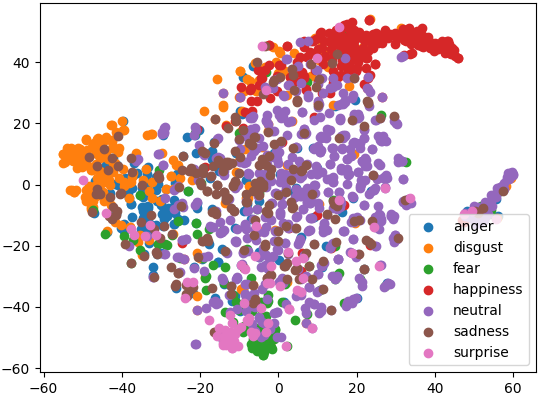
\includegraphics[width=\linewidth]{Images/Features/CE_5.png}
            \caption{Cross Entropy Loss}
            \label{CE_5}
        \end{subfigure}
        \begin{subfigure}{0.32\textwidth}
            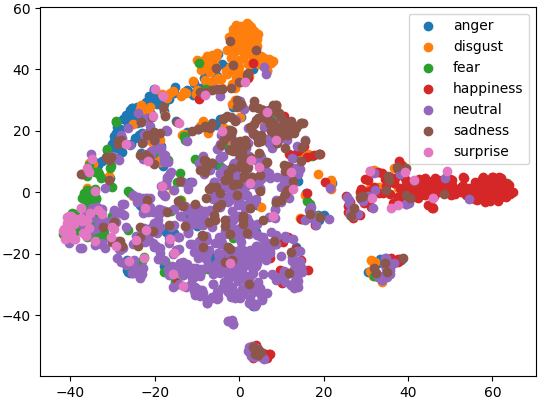
\includegraphics[width=\linewidth]{Images/Features/Center_5.png}
            \caption{Center Loss}
            \label{Center_5}
        \end{subfigure}
        \begin{subfigure}{0.32\textwidth}
            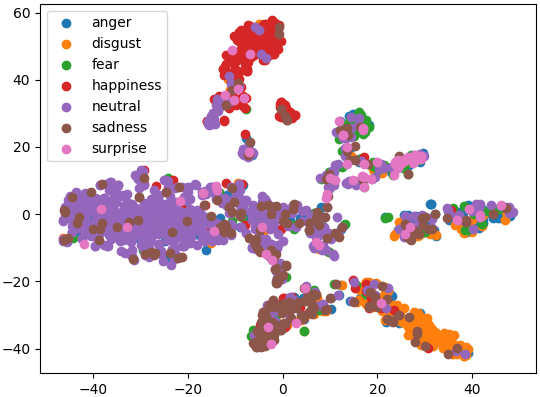
\includegraphics[width=\linewidth]{Images/Features/Island_5.png}
                \caption{Island Loss}
                \label{Island_5}
            \end{subfigure}
    \end{subfigure}
         \caption{t-SNE plot features of validation samples for different loss functions 10 epochs training.}
         \label{features_img}
\end{figure*}


\subsection{Dataset Merge}
As an additional experiment, CalD3rMenD3s, BU3DFE and Bosphorus datasets are merged into a single dataset for a final testing of the model. Whether it is true that CalD3rMenD3s is spontaneous while BU3DFE and Bosphorus are posed, the low intensity expressions from BU3DFE can be assimilated as spontaneous expression, while the overly exaggerated expressions both from BU3DFE and Bosphorus can be useful for the model to capture the most important features of the expressions and transfer that knowledge over less intense expressions.

    The final dataset is composed of 12098 images which distribution is shown in Figure \ref{Global_distribution} which is then split into a training set and a test set using 80\%-20\% policy. 
    Final results are shown in Table \ref{Global_results} with confusion matrix and training statistics in Figures \ref{Global_confusion} and \ref{Global_training}
    
    \begin{table}[H]
        \centering
        \caption{Results on Global dataset}
        \label{Global_results}
        \begin{tabular}{cccc}
        \hline
        Model & Year &Accuracy (\%) & Classes\\
        \hline
        \textbf{This} & 2024 & 68,48 & 7 \\
        \hline
        \end{tabular}
    \end{table}

    \begin{figure}[H]
        \centering
        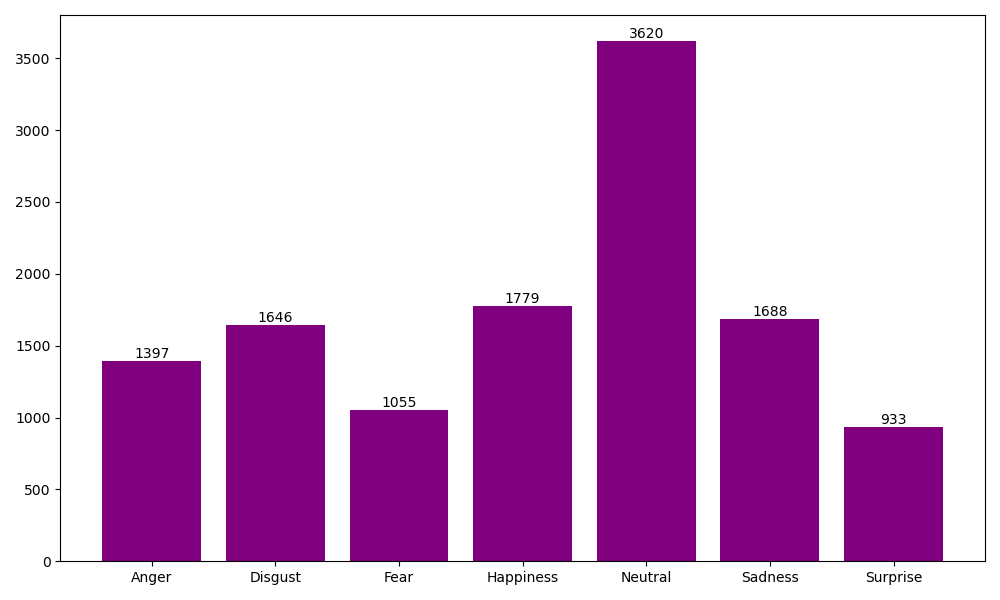
\includegraphics[width=1\columnwidth]{Images/Plot1.png}
        \caption{Classes distribution of the Global dataset}
        \label{Global_distribution}
    \end{figure}
    
  

\begin{figure*}[ht]
    \centering
    % First row
    \begin{subfigure}{\textwidth}
        \centering
        \begin{subfigure}{0.32\textwidth}
            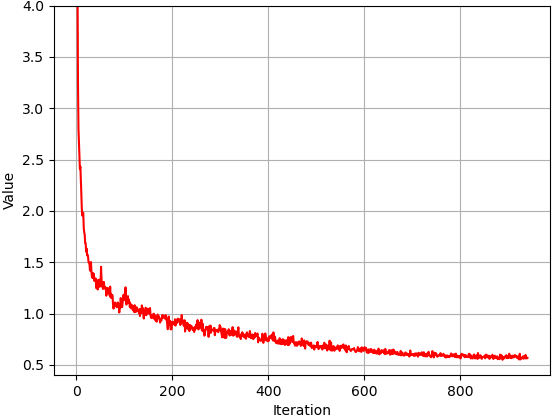
\includegraphics[width=\linewidth]{Images/training/Global_7_train_loss.png}
            \caption{Training Loss}
            \label{Global_7_train_loss}
        \end{subfigure}
        \begin{subfigure}{0.32\textwidth}
            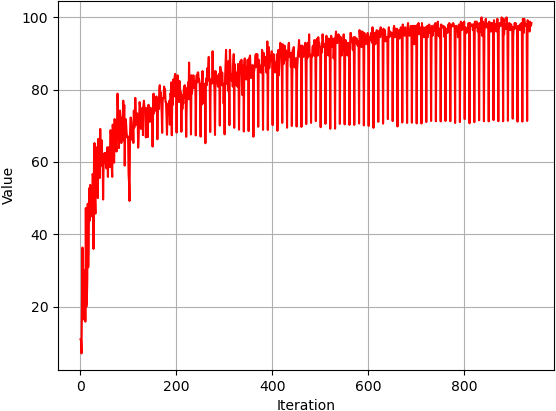
\includegraphics[width=\linewidth]{Images/training/Global_7_train_acc.png}
            \caption{Training Accuracy}
            \label{Global_7_train_acc}
        \end{subfigure}
        \begin{subfigure}{0.32\textwidth}
            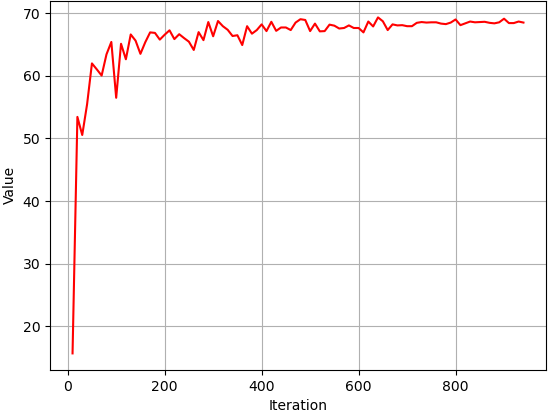
\includegraphics[width=\linewidth]{Images/training/Global_7_val_acc.png}
            \caption{Validation Accuracy}
            \label{Global_7_val_acc}
        \end{subfigure}
    \end{subfigure}
    \caption{Training and Validation Statistics for the Global dataset 7 classes}
    \label{Global_training}
\end{figure*}
    
\begin{figure}[H]
    \centering
    % First row
    \begin{subfigure}{0.37\textwidth}
        \centering
        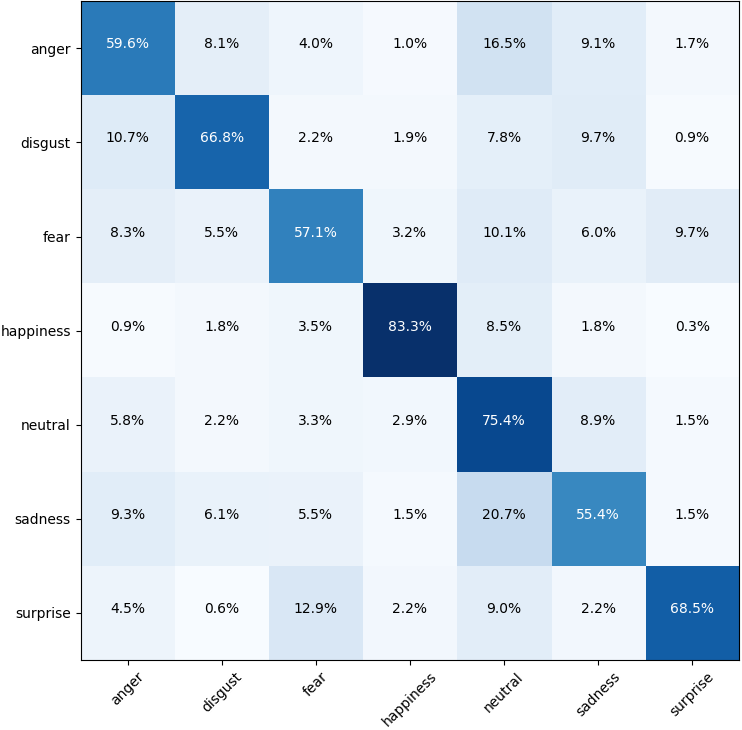
\includegraphics[width=\linewidth]{Images/conf_mat/conf_mat_Global_7.png}
        \caption{Confusion Matrix. \footnotesize{X-axis: predicted class, Y-axis: true class}}
        \label{conf_mat_Global_7}
    \vspace{0.15cm}
    \end{subfigure}
    \hspace{0.05\textwidth} % Add space between the subfigures
    \begin{subfigure}{0.39\textwidth}
        \centering
        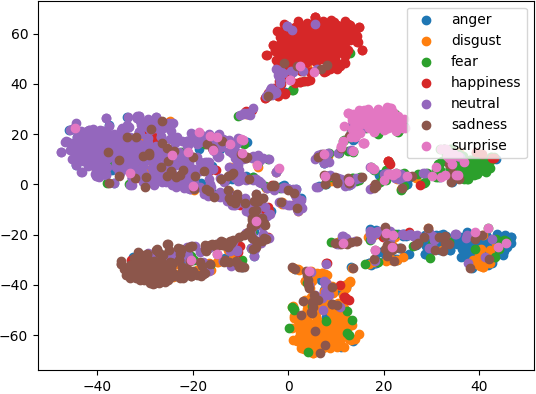
\includegraphics[width=\linewidth]{Images/Features/feat_Global_7.png}
        \caption{Features}
        \label{feat_Global_7}
    \end{subfigure}
    \caption{Training results on Global dataset 7 classes}
    \label{Global_confusion}
\end{figure}
        


